\documentclass[11pt]{beamer}
\mode<presentation>
\usepackage{amssymb,textcomp}
%\usepackage{beamerthemesplit}
\usepackage{beamerthemeJuanLesPins}
\usepackage{verbatim}
\usepackage[ruled,vlined]{algorithm2e}
\usepackage{tikz}
\usetikzlibrary{calc}
\usepackage{subcaption}
\usefonttheme{serif}
\title{Autovalores y Autovectores.}
\author{Jos\'e Luis Ram\'irez B.}
\date{\today}
\begin{document}
\frame{\titlepage}
\frame{\tableofcontents}
\section{Introducci\'on}
\begin{frame}{Introducci\'on.}
  \begin{itemize}
    \item<1-> El estudio de los autovalores de sistemas surge por doquier en muchas \'areas de la 
   ciencia, ingenier\'ia, econom\'ia ...
   \begin{itemize}
      \item<2-> An\'alisis de estructuras
      \item<3-> Dise\~no de sistemas electr\'onicos
      \item<4-> An\'alisis de sistemas el\'ectricos:
      \begin{itemize}
         \item<5-> Sincronismo del sistema productor
         \item<6-> Estabilidad del sistema ante perturbaciones
         \item<7-> Planificaci\'on nuevo equipo
         \item<8-> Otros muchos
      \end{itemize}
      \item<9-> Mercados financieros.
   \end{itemize}
   \item<10-> Es tambi\'en muy importante para analizar el comportamiento de m\'etodos num\'ericos.
   \end{itemize}
\end{frame}
  %%%%%%%
  \begin{frame}{Formulaci\'on del Problema.}
    \begin{block}{Definici\'on:}
       Dada una matriz $A \in \mathbb{C}^{n \times n}$, calcular un valor $\lambda \in \mathbb{C}$ y un 
    vector $x$ no nulo tales que
    $$
    Ax = \lambda x
    $$
    \end{block}
    \begin{itemize}
    \item<2-> A $\lambda$ se le denomina autovalor o valor propio y a $x$ su correspondiente vector 
    propio o autovector.
    \item<3-> Para que exista una soluci\'on distinta de la trivial, $x = 0$, el valor propio $\lambda$ 
    deber\'a ser ra\'iz del polinomio de grado $n$, polinomio caracter\'istico:
    $$
    \det(A - \lambda I) = 0
    $$
    \end{itemize}
    \end{frame}
    %%%%%%
\begin{frame}
  \begin{block}{Definici\'on:}
     Se denomina espectro de la matriz $A$ , $\sigma(A)$, al conjunto de
  los valores propios de $A$. Es decir,
  $$
  \sigma(A) = \{\lambda \in \mathbb{C}: \det(A - \lambda I) = 0\}.
  $$
  \end{block}
  \uncover<2->{
  \begin{block}{Definici\'on:}
     Se denomina radio espectral, $\rho(A)$, de una matriz $A$ de orden
  $n$, al valor m\'aximo de los m\'odulos de los valores propios de la matriz:
  $$
  \rho(A) = \max_{\lambda_i \in \sigma(A)} |\lambda_i|$$
  \end{block}}
  \begin{itemize}
     \item<3-> El radio espectral de una matriz es el radio del menor c\'irculo del plano complejo centrado en el origen que contiene a todos los valores propios de la matriz.
  \end{itemize}
  \end{frame}
  %%%%%%
\begin{frame}{Propiedades.}
  \begin{itemize}
     \item<1-> $A$ y $A^t$ poseen los mismos autovalores.
  \item<2-> $A=A^t$ implica  que todos sus autovalores son reales.
  \item<3-> $A$ es inversible si y s\'olo si $\lambda \neq 0, \forall \lambda$ autovalor de $A$.
  \item<4-> $A$ inversible  y $\lambda$ autovalor de $A$ entonces $1/\lambda$ es autovalor de $A^{-1}$.
  \item<5-> $tr(A) = \sum\lambda_i$, $\det(A) = \prod \lambda_i$
  \end{itemize}
  \end{frame}
  %%%%%%
  \begin{frame}{Localizaci\'on de valores propios.}
    \begin{itemize}
       \item Si no se necesita calcular exactamente los valores propios, sino saber, en cierta medida,  
    d\'onde se encuentran en el plano complejo, existen varias formas de hacerlo.
    \item<2->  La m\'as simple surge de la relaci\'on
    $$
    |\lambda| \leq \|A\|
    $$
    para cualquier norma matricial inducida por una norma vectorial.
    \item<3-> Los valores propios de una matriz se localizan en el plano
    complejo, dentro del c\'irculo centrado en el origen de radio $\|A\|$.
    \end{itemize}
    \end{frame}
    %%%%%%
    \begin{frame}{Localizaci\'on de valores propios.}
    \begin{block}{Teorema: C\'irculos de Gershgorin}
       Sea $A \in \mathbb{C}^{n \times n}$ y definiendo los c\'irculos de Gershgorin
    como los conjuntos
    $$
    R_i = \left\{z \in \mathbb{C} / |z-a_{ii}| \leq \sum_{\substack{j=1 \\ j\neq i}}^n 
    |a_{ij}|\right\}
    $$
    entonces el espectro de $A$ es subconjunto de la uni\'on de los c\'irculos, esto es:
    $$
    \sigma(A) \subseteq \bigcup_{i=1}^nR_i = S_R 
    $$
    \end{block}
    \end{frame}
    %%%%%%
    \begin{frame}
    \begin{itemize}
       \item<1-> Escribiendo $A=D+P$, donde $D$ es diagonal y est\'an los elementos de la
    diagonal de $A$, por lo tanto $p_{ii} = 0 \forall i$.
    \item<2-> Considerando $\lambda \in \sigma(A)$, $\lambda \neq a_{ii}$ y definiendo la
    matriz $B_{\lambda} = A - \lambda I = (D - \lambda I) + P$
    \item<3-> Dado que $B$ es singular, por lo tanto existe un vector no nulo $x$ tal que $B_{\lambda}x 
    = 0$, por lo tanto $(( D - \lambda I ) + P ) x = 0$, luego $x = -( D - \lambda I )^{-1}Px$ 
    aplicando $\|\cdot\|_{\infty}$ a ambos de la igualdad
    $$
    \|x\|_{\infty} \leq \|(D-\lambda I)^{-1}\|_{\infty}\|P\|_{\infty}\|x\|_{\infty}
    $$
    $$
    1 \leq \|(D-\lambda I)^{-1}\|_{\infty}\|P\|_{\infty} = \sum_{\substack{j=1 \\ j \neq 
    k}}^n\dfrac{|p_{kj}|}{|a_{kk}-\lambda|} = \sum_{\substack{j=1 \\ j \neq 
    k}}^n\dfrac{|a_{kj}|}{|a_{kk}-\lambda|}
    $$
    es decir $\lambda$ satisface la condici\'on de pertenencia al c\'irculo $R_k$. Por lo tanto si se 
    unen todos los c\'irculos con seguridad los autovalores estar\'an dentro del conjunto resultante.
    \end{itemize}
    \end{frame}
    %%%%%%
    \begin{frame}
    \begin{block}{Teorema:}
    $A$ y $A^t$ tienen el mismo espectro (a los circulos de $A^t$ los denotaremos por $C_i$ luego 
    $\bigcup_{i = 1}^n C_i = S_C$).
    \end{block}
    \uncover<2->{
    \begin{block}{Teorema:}
       $$
       \forall \lambda \in \sigma(A) \rightarrow \lambda \in S_R \cap S_C
       $$
    \end{block}}
    \end{frame}
    %%%%%%
    \begin{frame}{Ejemplo:}    
      \begin{itemize}
      \item<1-> Dada la matriz $A= \dfrac{1}{16}\left[\begin{array}{ccc}
        -8 & -2 & 4 \\
        -1 & 6 & 2 \\
        2 & 2 & -10      
      \end{array}\right]$
      \item<2-> Note que $\|A\| = (1/16)\max{14,9,14} = 7/8$ de modo que los valores propios de $A$ cumplen con $|\lambda| \leq 7/8$.
      \item<3-> Se Puede mejorar este estimado con el Teorema de Gershgorin.
      \item Tenemos que $r_1 =3/8$, $r_2 = 3/16$, $r_3 = 1/4$. Los discos son:
      \begin{align*}
      R_1 & = \{ z \in \mathbb{C} / |z+1/2|\leq 3/8\}, \Rightarrow -7/8 \leq z \leq -1/4\\
      R_2 & = \{ z \in \mathbb{C} / |z-3/8|\leq 3/16\}, \Rightarrow 3/16 \leq z \leq 9/16\\
      R_3 & = \{ z \in \mathbb{C} / |z+5/8|\leq 1/4\}, \Rightarrow -7/8 \leq z \leq -3/8
      \end{align*}
      \end{itemize}      
    \end{frame}
    %%%%%%
    \begin{frame}{Gershgorin Circles}
      \begin{figure}[ht]
          \centering
          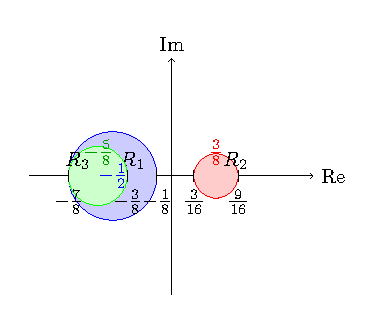
\includegraphics[width=0.7\textwidth]{prueba.pdf} % Adjust width as needed
          \caption{C\'irculos de Gerschgorin para la matriz $A$.}
      \end{figure}
  \end{frame}
    %%%%%%
    \begin{frame}{Ejemplo:}
      \begin{itemize}
        \item La matriz $A$ es no singular ya que el cero esta fuera de los c\'irculos.
        \item Hay un autovalor en $R_2$ y los otros dos est\'an en $R_1 \cup R_3$.
        \item Se puede hacer el mismo an\'alisis para la matriz $A^t$ y obtener otra familia de c\'irculos $R_1',R_2', R_3'$.
        $$
        A^t = \dfrac{1}{16}\left[\begin{array}{ccc}
          -8 & -1 & 2 \\
          -2 & 6 & 2 \\
          4 & 2 & -10      
        \end{array}\right]
        $$
        \item Se tiene que $r_1' = r_1$, $r_2' = r_2$, $r_3' = r_3$. Los discos son:
        \begin{align*}
        R_1' & = \{ z \in \mathbb{C} / |z+1/2|\leq 3/16\}, \Rightarrow -11/16 \leq z \leq -5/16\\
        R_2' & = \{ z \in \mathbb{C} / |z-3/8|\leq 1/4\}, \Rightarrow 1/8 \leq z \leq 5/8\\
        R_3' & = \{ z \in \mathbb{C} / |z+5/8|\leq 3/8\}, \Rightarrow -1 \leq z \leq -1/4
        \end{align*}
      \end{itemize}
    \end{frame}
    %%%%%%
    \begin{frame}{C\'irculos de Gershgorin - $A$ y $A^t$}
      \begin{figure}
        \centering
        \begin{subfigure}{0.48\textwidth}
          \centering
          \begin{tikzpicture}[scale=2]
            % Define the centers and radii of the circles for A
            \def\centerROne{-0.5}
            \def\radiusROne{0.375}
            \def\centerRTwo{0.375}
            \def\radiusRTwo{0.1875}
            \def\centerRThree{-0.625}
            \def\radiusRThree{0.25}
    
            % Draw the axes
            \draw[->] (-1.2,0) -- (1.2,0) node[right] {Re};
            \draw[->] (0,-1) -- (0,1) node[above] {Im};
    
            % Draw the circles
            \draw[blue,fill=blue!20] (\centerROne,0) circle (\radiusROne) node[above right, black] {$R_1$};
            \draw[red,fill=red!20] (\centerRTwo,0) circle (\radiusRTwo) node[above right,black] {$R_2$};
            \draw[green,fill=green!20] (\centerRThree,0) circle (\radiusRThree) node[above left, black] {$R_3$};
    
            % Mark the boundaries of the intervals on the real 
            {\tiny
            \foreach \x/\xtext in {-0.875/-\frac{7}{8}, -0.125/-\frac{1}{8}, 0.1875/\frac{3}{16}, 0.5625/\frac{9}{16}, -0.375/-\frac{3}{8}, -0.375/-\frac{3}{8}}
            {
              \draw (\x,0.05) -- (\x,-0.05) node[below] {$\xtext$};
            }}
    
            % Add some labels for the centers
            \node[blue] at (\centerROne,0) {$-\frac{1}{2}$};
            \node[red] at (\centerRTwo,0.2) {$\frac{3}{8}$};
            \node[green!60!black] at (\centerRThree,0.2) {$-\frac{5}{8}$};
          \end{tikzpicture}
          \caption{C\'irculos de Gershgorin para $A$}          
        \end{subfigure}
        \hfill
        \begin{subfigure}{0.48\textwidth}
          \centering
          \begin{tikzpicture}[scale=2]
            % Define the centers and radii of the circles for At
            \def\centerROne{-0.5}
            \def\radiusROne{0.1875}
            \def\centerRTwo{0.375}
            \def\radiusRTwo{0.25}
            \def\centerRThree{-0.625}
            \def\radiusRThree{0.375}
    
            % Draw the axes
            \draw[->] (-1.2,0) -- (1.2,0) node[right] {Re};
            \draw[->] (0,-1) -- (0,1) node[above] {Im};
    
            % Draw the circles        
            \draw[red,fill=red!20] (\centerRTwo,0) circle (\radiusRTwo) node[above right,black] {$R_2'$};        
            \draw[green,fill=green!20] (\centerRThree,0) circle (\radiusRThree) node[above left, black] {$R_3'$};
            \draw[blue,fill=blue!20] (\centerROne,0) circle (\radiusROne) node[above right, black] {$R_1'$};
    
            % Mark the boundaries of the intervals on the real axis
            {\tiny
              \foreach \x/\xtext in {-1/-1, -0.6875/-\frac{11}{16}, -0.3125/-\frac{5}{16}, 0.125/\frac{1}{8}, 0.625/\frac{5}{8}, -0.25/\;\;\quad\quad-\frac{1}{4}}
            {
              \draw (\x,0.05) -- (\x,-0.05) node[below] {$\xtext$};
            }}
    
            % Add some labels for the centers
            \node[blue] at (\centerROne,0) {$-\frac{1}{2}$};
            \node[red] at (\centerRTwo,0.2) {$\frac{3}{8}$};
            \node[green!60!black] at (\centerRThree,0.2) {$-\frac{5}{8}$};
    
          \end{tikzpicture}
          \caption{C\'irculos de Gershgorin para $A^t$}          
        \end{subfigure}
        \caption{C\'irculos de Gershgorin para $A$ y $A^t$}        
      \end{figure}
    \end{frame}
    %%%%%%
    \begin{frame}{Ejemplo:}
      \begin{itemize}
        \item<1-> Se sabe que los autovalores de $A$ y $A^t$ coinciden, por tanto
        la intersecci\'on de $(R_1\bigcup R_2\bigcup R_3) \bigcap (R_1' \bigcup R_2' \bigcup R_3')$ nos da un refinamiento.
        \item<2-> Unión de c\'irculos de $A$: 
        \begin{itemize}
          \item $R_1: [-7/8,-1/4]$
          \item $R_2: [3/16,9/16]$
          \item $R_3: [-7/8,-3/8]$
        \end{itemize}
        {\centering Union: $[-7/8,-1/4]\cup[3/16,9/16]$}
        \item<3-> Unión de c\'irculos de $A^t$:
        \begin{itemize}
          \item $R_1': [3/16,9/16]$
          \item $R_2': [1/8,5/8]$
          \item $R_3': [3/16,9/16]$
        \end{itemize}
        {\centering Union: $[-1,-1/4]\cup[1/8,5/8]$}         
      \end{itemize}
    \end{frame}
    %%%%%%
    \begin{frame}{Ejemplo:}
      \begin{itemize}
        \item<1-> Intersecci\'on de las uniones: $[-7/8,-1/4]\cup[3/16,9/16]$.
        \item<2-> Esto significa que todos los autovalores de $A$ y $A^t$ deben estar contenidos en los intervalos $[-7/8,-1/4]$ (negativos) y $[3/16,9/16]$ (positivos).
        \item<3-> No hay autovalores en los intervalos $[-1,-7/8)$ ni $(9/16,5/8]$.
        \item<4-> La matriz $A$ no es simétrica , ya que los radios de los discos de $A$ y $A^t$ son diferentes.
        \item<5-> Todos los autovalores son reales, debido a que los discos están contenidos en la recta real.
        \item<6-> La matriz es invertible, ya que 0 no está en ningún disco de Gerschgorin.
      \end{itemize}
    \end{frame}
    %%%%%%
    \section{M\'etodo de las Potencias}
    \begin{frame}{M\'etodo de las Potencias}
      \begin{itemize}
        \item El objetivo de este m\'etodo es hallar $\lambda_1$ autovalor de $A$ y un autovector $x$ asociado a $\lambda_1$.
        \item<2-> Supongamos que $A \in \mathbb{R}^{n \times n}$ posee $n$ autovalores $\lambda_1,\lambda_2,\ldots,\lambda_n$ y $n$ autovectores asociados $v^{(1)},v^{(2)},\ldots,v^{(n)}$, tales que:
        $$
        |\lambda_1|>|\lambda_2|\geq\cdots\geq|\lambda_n|
        $$
        entonces, $|\lambda_1|>|\lambda_j|\forall j=2,\ldots,n$ y $\{v^{(j)}\}$ es un conjunto de vectores linealmente independientes.
      \end{itemize}
    \end{frame}
    %%%%%%
    \begin{frame}{M\'etodo de las Potencias}
      \begin{itemize}
        \item Si $x$ es un vector cualquiera en $\mathbb{R}^n$, el hecho de que $\{v^{(j)}\} \forall j=1,\ldots,n$ sea linealmente independiente, implica
        que existen constantes $\alpha_1, \alpha_2,\ldots,\alpha_n$ tal que:
        \begin{align*}
          x &= \sum_{j=1}^n\alpha_jv^{(j)}\\
          \uncover<2->{Ax &= \sum_{j=1}^n\alpha_jAv^{(j)} = \sum_{j=1}^n\alpha_j\lambda_jv^{(j)}\\}
          \uncover<3->{A^2x &= A(Ax) =\sum_{j=1}^n\alpha_j\lambda_jAv^{(j)} = \sum_{j=1}^n\alpha_j\lambda_j^2v^{(j)}\\}
          \uncover<4->{A^kx &= A^{(k-1)}(Ax) = \sum_{j=1}^n\alpha_j\lambda_j^kv^{(j)}}
          \end{align*}
        \end{itemize}
    \end{frame}    
    %%%%%%
    \begin{frame}{M\'etodo de las Potencias}
      \begin{itemize}
        \item Dado que
        $$
          |\lambda_1|>|\lambda_j|\forall j=2,\ldots,n \Rightarrow \left|\frac{\lambda_j}{\lambda_1}\right|<1 \Rightarrow \left|\frac{\lambda_j}{\lambda_1}\right|^k\xrightarrow{\forall j=2,\ldots,n}0
          $$

          $$
          \sum_{j=1}^n\alpha_j\lambda_j^kv^{(j)} = \lambda_1^k\sum_{j=1}^n\alpha_j\left|\frac{\lambda_j}{\lambda_1}\right|^kv^{(j)} \Rightarrow \lim_{k \to \infty}A^kx = \lim_{k \to \infty}\alpha_1\lambda_1^kv^{(1)}
          $$
          \item<2-> Esta sucesi\'on converge a cero si $|\lambda_1|<1$ y diverge si $|\lambda_1|>1$ siempre que $\alpha_1\neq 0$.
          \item<3-> De esta \'ultima expresi\'on se obtiene la manera de escalar las potencias de $A^kx$ para que el l\'imite sea finito y distinto de cero.
          \end{itemize}
      \end{frame}
    %%%%%%
    \begin{frame}{M\'etodo de las Potencias}
      \begin{itemize}
        \item Para escalar las potencias se inicia eligiendo un vector $x^{(0)}$ tal que $x_{p_0}^{(0)}=1=\|x^{(0)}\|_{\infty}$.
        \item<2-> Sea $y^{(1)}=Ax^{(0)}=\sum_{j=1}^n\alpha_j\lambda_jv^{(j)}$ y sea $\mu^{(1)}=y_{p_0}^{(1)}$, eventualmente $\mu^{(k)}\to \lambda_1$
        {\small
        \begin{align*}
\mu^{(1)} &= y_{p_0}^{(1)} = \frac{y_{p_0}^{(1)}}{x_{p_0}^{(0)}}\\
& = \displaystyle\frac{\alpha_1\lambda_1v_{p_0}^{(1)}+\displaystyle\sum_{j=2}^n\alpha_j\lambda_jv_{p_0}^{(j)}}{\alpha_1v_{p_0}^{(1)}+\displaystyle\sum_{j=2}^n\alpha_jv_{p_0}^{(j)}} = \lambda_1\left(\displaystyle\frac{\alpha_1v_{p_0}^{(1)}+\displaystyle\sum_{j=2}^n\alpha_j\left|\frac{\lambda_j}{\lambda_1}\right|v_{p_0}^{(j)}}{\alpha_1v_{p_0}^{(1)}+\displaystyle\sum_{j=2}^n\alpha_jv_{p_0}^{(j)}}\right)
\end{align*}}
        
      \end{itemize}
    \end{frame}
    %%%%%%
    \begin{frame}{M\'etodo de las Potencias}
      \begin{itemize}
        \item<1-> Sea $p_1$ el entero m\'as peque\~no tal que $|y_{p_1}^{(1)}|=\|y^{(1)}\|_{\infty}$ y sea
        $$
        x^{(1)} = \frac{y^{(1)}}{y_{p_1}^{(1)}} = \frac{Ax^{(0)}}{y_{p_1}^{(1)}} \Rightarrow \|x^{(1)}\|_{\infty} = 1 = |x_{p_1}^{(1)}|
        $$
        \item<2-> Se define a continaci\'on
        $$
        y^{(2)} = Ax^{(1)} = \frac{A^2x^{(0)}}{y_{p_1}^{(1)}}
        $$
        \item<3-> Sea
        $$
        \mu^{(2)} =  y_{p_1}^{(2)} =  \frac{y_{p_1}^{(2)}}{x_{p_1}^{(1)}} = \frac{\lambda_1^2\left(\displaystyle\frac{\alpha_1v_{p_1}^{(1)}+\sum_{j=2}^n\alpha_j\left|\frac{\lambda_j}{\lambda_1}\right|^2v_{p_1}^{(j)}}{y_{p_1}^{(1)}}\right)}{\lambda_1\left(\displaystyle\frac{\alpha_1v_{p_1}^{(1)}+\sum_{j=2}^n\alpha_j\left|\frac{\lambda_j}{\lambda_1}\right|v_{p_1}^{(j)}}{y_{p_1}^{(1)}}\right)}
        $$
      \end{itemize}
    \end{frame}
    %%%%%%
    \begin{frame}{M\'etodo de las Potencias}
      \begin{itemize}
        \item As\'i sucesivamente. Los sucesivos vectores $x^{(k)}$, $y^{(k)}$ y los escalares $\mu^{(k)}$ siendo
        $$
        y^{(k)} = Ax^{(k-1)}
        $$        
        $$
        \mu^{(k)} = y_{p_{k-1}}^{(k)} = \lambda_1\left(\frac{\alpha_1v_{p_{k-1}}^{(1)}+\sum_{j=2}^n\alpha_j\left|\frac{\lambda_j}{\lambda_1}\right|^kv_{p_{k-1}}^{(j)}}{\alpha_1v_{p_{k-1}}^{(1)}+\sum_{j=2}^n\alpha_j\left|\frac{\lambda_j}{\lambda_1}\right|^{k-1}v_{p_{k-1}}^{(j)}}\right)
        $$
        y
        $$
        x^{(k)} = \frac{y^{(k)}}{y_{k}^{(k)}} = \frac{A^kx^{(0)}}{y_{p_1}^{(1)} y_{p_2}^{(2)} \cdots y_{p_k}^{(k)}}
        $$
        donde $p_k$ es el entero m\'as peque\~no para el cual $|y_{p_k}^{(k)}|=\|y^{(k)}\|_{\infty}$.
      \end{itemize}
    \end{frame}
    %%%%%%
    \begin{frame}{M\'etodo de las Potencias}
      \begin{itemize}
        \item<1-> De esta manera, se tiene que:
        $$
        \lim_{k \to \infty}\mu^{(k)} = \lambda_1
        $$        
        $$
        x^{(0)} = \alpha_1v^{(1)} + \alpha_2v^{(2)}+\cdots+\alpha_nv^{(n)}
        $$
        \item<2-> Suponiendo que $\alpha_1 \neq 0$ entonces del m\'etodo de la potencia se obtiene $\mu^{(k)}\to\lambda_1$ y $x^{(k)}\to x$  autovector asociado a $\lambda_1$.
        \item<3-> La velocidad de convergencia del m\'etodo depende de la magnitud del cociente $\frac{\lambda_2}{\lambda_1}$. Cuanto m\'as cercano a 1 sea el cociente m\'as lenta ser\'a la convergencia.
      \end{itemize}
    \end{frame}
    %%%%%%
    \begin{frame}{M\'etodo de las Potencias}
\begin{algorithm}[H] 
  \footnotesize
 \SetKwInOut{Input}{input}
 \SetKwInOut{Output}{output}
 \caption{Algoritmo de Potencia.}
 \Input{$A \in \mathbb{R}^{n \times n}$, $x \in \mathbb{R}^n$, N\'umero m\'aximo de iteraciones $N$, tolerancia $TOL$.}
 \Output{autovalor aproximado $\mu$ y autovector asociado $x$ con $\|x\|_{\infty}=1$.} 
 Hallar $p$  con $1\leq p \leq n$ tal que $|x_p|=\|x\|_{\infty}$\\
 $x=\dfrac{x}{x_p}$\\
 \For{$k\leftarrow 1$ \KwTo $N$}
 {
  $y \leftarrow Ax$; $\mu \leftarrow y_p$\\
  Hallar $p$  con $1\leq p \leq n$ tal que $|y_p|=\|y\|_{\infty}$\\
  \If{$y_p=0$}
  {
    Salida $(autovalor,autovector) = (0,x)$;  
    Seleccionar nuevo $x$ y reiniciar; EXIT
  }
  $err \leftarrow \|x-y/y_p\|_{\infty}$; 
  $x=\dfrac{y}{y_p}$\\
  \If{$err<TOL$}
  {
    Salida ($\mu$,$x$)
    EXIT
  }
 } 
\end{algorithm}
  \end{frame}
    %%%%%%
    \begin{frame}{Ejemplo}
      Sea la matriz $A=\left(\begin{array}{ccc}
        4 & -1& 1\\
-1 & 3 & -2\\
1 & -2 & 3\\
       \end{array}\right)$ y el vector $x^{(0)}=\left(\begin{array}{c}
        1\\0\\0\\\end{array}\right)$   
    Se obtienen los siguientes resultados:\\[10pt]
    {\scriptsize
    \begin{tabular}{|c|c|c|c|c|c|c|}\hline
      $k$ & 0 & 1 & 2 & 3 & $\cdots$ & 14\\\hline
      $x^{(k)}$ & $\left(\begin{array}{c}1\\0\\0\\\end{array}\right)$ & $\left(\begin{array}{c}1\\-0.25\\0.25\\\end{array}\right)$ & $\left(\begin{array}{c}1\\-0.5\\0.5\\\end{array}\right)$ & $\left(\begin{array}{c}1\\-0.70\\0.70\\\end{array}\right)$ & $\cdots$ & $\left(\begin{array}{c}1\\-0.9998\\0.9998\\\end{array}\right)$\\\hline
      $\mu^{(k)}$ & -- & 4 & 4.5 & 5.0 & $\cdots$ & 5.9993\\\hline
    \end{tabular}}\\[10pt]
    Parece que el valor propio dominante va a ser $\lambda = 6$ y su vector propio asociado $(1,-1,1)$.
  \end{frame}
  \end{document}
